\documentclass[handout]{beamer} 
%\setbeamercolor{alerted text}{fg=green}
\setbeamercolor{frametitle}{bg=red!40!black}
\setbeamercolor{structure}{fg=black}

\setbeamercolor{item}{fg=green}
\geometry{paperwidth=140mm,paperheight=105mm}
\usepackage{helvet}
\usefonttheme{serif}     % Font theme: serif
\usepackage{ccfonts}     % Font family: Concrete Math
\usepackage[T1]{fontenc} % Font encoding: T1





% theme split
\usepackage{beamerthemesplit}
\usepackage{amsmath,thmtools}
% theme shadow
\usepackage[font=normalsize,labelfont=bf]{caption}
\usepackage{beamerthemeshadow}
\usepackage [english]{babel}
\usepackage [autostyle, english = american]{csquotes}
\MakeOuterQuote{"}

\begin{document}
% sf family, bold font
\sffamily \bfseries

\title
[ Cashless Economy 
\hspace{0.5cm}
\insertframenumber/\inserttotalframenumber]
{Cashless Economy}
\author
[DUBALE AMOL J.]
{Presented by \\ DUBALE AMOL J.  \\
}
\date{ Guided by : Prof. S. A. THANEKAR  \\
\vspace{0.2cm}

  Department of Computer Engineering \\
 Amrutvahini College of Engineering , Sangamner \\
  \vspace{1.2cm}
  05/04/2017
  }
  
\logo{
\includegraphics[height=1.5cm]{avlogo.png}}  
  
  
%%%%%%%%%%%%%%%%%%%%%%%%%%%%%%%%%%
\begin{frame}
   \titlepage
 \end{frame}
%%%%%%%%%%%CHANGE NEEDED BELOW
\begin{frame}
\frametitle{Contents:}
\begin{enumerate}

\item Introduction
\item Objectives
\item Motivation
\item Literature Survey
\item Credit Card Payment System
\item EVM Payment System
\item NFC Payment System
\item Apple-Pay
\item E-VALLET
\item Conclusion
\item References
\end{enumerate}
\end{frame}
%%%%%%%%%%%%%%%%%%%%%%%%%%%%
\frame{\frametitle{Introduction : }
\begin{figure}[h]
\begin{center}
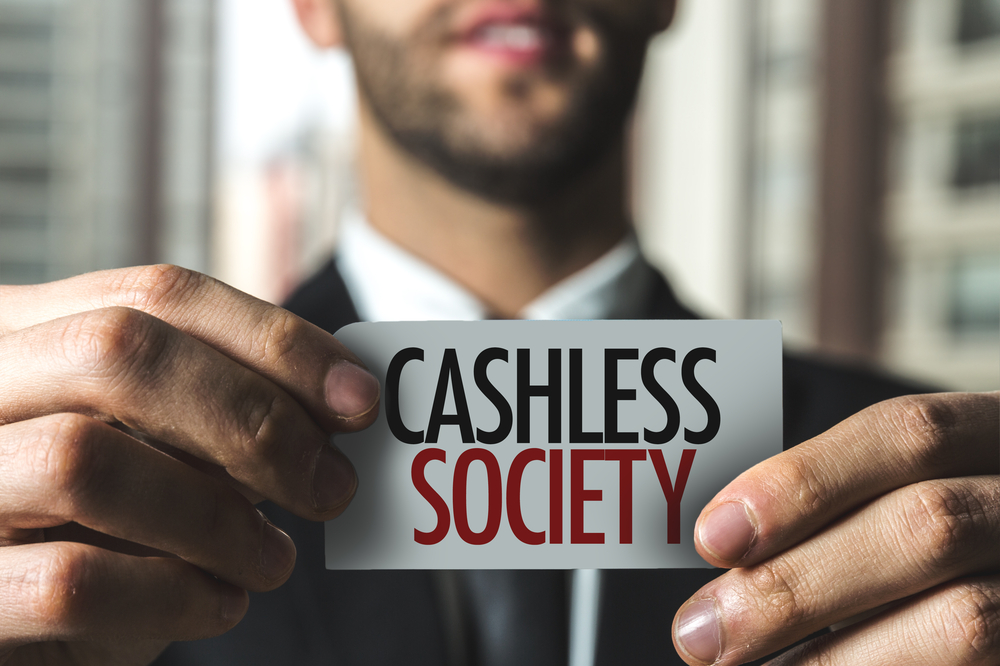
\includegraphics[scale=0.5,angle=360]{cashless1.jpg}
\caption{Cashless Society }
\end{center}
\end{figure}

\begin{itemize}
\item An economic state whereby financial transactions are not conducted with money in the form of physical banknotes or coins, but rather through the transfer of digital information between the transacting parties.\\
%\vspace{.4cm}
\item A cashless economy is one in which all the transactions are done using cards or digital means. The circulation of physical currency is minimal.

\end{itemize}
}
%%%%%%%%%%%%%%%%%%%%%%%%%%%%%%%%%%%%%%%%%
\frame{\frametitle{Objectives : } 
\begin{itemize}
\item Introduction of universal payment systems.
\item To curb generation of black money and corruption.
\item To reduce tax avoidance and money laundering.
\item To reduce the difficulties in transporting the money.
\item Minimization of the wastage of money in printing of physical notes, coins.
\end{itemize}
}
%%%%%%%%%%%%%%%%%%%%%%%%%%%%%%%%%%%%%%%%%%%%%
\frame{\frametitle{Motivation : }
\begin{itemize}
\item Generation of black money and Increased corruption by physical cash. 
\item Criminal activities related to cash(money laundering, robberies etc).
\item Long lasting bank transactions.
\end{itemize}
}
%%%%%%%%%%%%%%%%%%%%%%%%%%%%%%%%%%%%%%%%%%%%
\frame{\frametitle{Literature Survey : }
\textbf{Paper 1}
\begin{itemize}
\item \textbf{Title : }\\
\lq\lq  Next Generation Smart Transaction Touch Points \rq\rq
\item \textbf{Name of authors : } K. V. Kuganathan, Gihan N.Wikramanayake
\item \textbf{Year of Publication : }2014
\end{itemize}
\textbf{Paper content : }
\begin{enumerate}
\item The provision of mobile application to perform banking transactions while enabling merchant payments through a SMART card.
\item The new local initiative for  mobile payments which will promote the acceptance and adoption of cashless payment mechanisms.
\end{enumerate}
}
%%%%%%%%%%%%%%%%%%%%%%%%%%%%%%%%%%%%%%%%%%%%
\frame{\frametitle{Literature Survey :(Conti...) }
\textbf{Paper 2}
\begin{itemize}
\item \textbf{Title : }\\
\lq\lq The Implementation of a full EMV Smartcard for a Point-of-Sale Transaction \rq\rq
\item \textbf{Name of authors : }Oludele Ogundele, Pavol Zavarsky, Ron Ruhl, Dale Lindskog.
\item \textbf{Year of Publication : }2012
\end{itemize}
\textbf{Paper content : }
\begin{enumerate}
\item  Technical standard for smart payment cards, payment terminals and automated teller machines.
\item Introduction of changes in payment card environment and point of sale terminal.
\end{enumerate}
}
%%%%%%%%%%%%%%%%%%%%%%%%%%%%%%%%%%%%%%%%%%%%
\frame{\frametitle{Literature Survey :(Conti...) }
\textbf{Paper 3}
\begin{itemize}
\item \textbf{Title : }\\
\lq\lq IDA-Pay: an innovative micro-payment system based on NFC technology for Android               						  mobile devices \rq\rq
\item \textbf{Name of authors : }Luca Mainetti, Luigi Patrono, Roberto Vergallo.
\item \textbf{Year of Publication : }2014
\end{itemize}
\textbf{Paper content : }
\begin{enumerate}
\item  The evolution of modern mobile devices towards novel Radio Frequency (RF) capabilities, such as Near Field Communication (NFC).
\item  An  innovative  and  secure  NFC  micro-payment  system  based on peer-to-peer NFC operating mode for Android mobile phones.

\end{enumerate}
}
%%%%%%%%%%%%%%%%%%%%%%%%%%%%%%%%%%%%%%%%%%%%

\frame{\frametitle{Literature Survey :(Conti...) }
\textbf{Paper 4}
\begin{itemize}
\item \textbf{Title : }\\
\lq\lq  E-WALLET Properties  \rq\rq
\item \textbf{Name of authors : } Mia Olsen, Jonas Hedman and Ravi Vatrapu.
\item \textbf{Year of Publication : }2014
\end{itemize}
\textbf{Paper content : }
\begin{enumerate}
\item  intention  to  replace  the existing  physical  wallet,  with  its  notes,  coins,  photos,  plastic cards, loyalty cards etc.
  

\end{enumerate}
}
%%%%%%%%%%%%%%%%%%%%%%%%%%%%%%%%%%%%%%%%%%%%

























%%%%%%%%%%%%%%%%%%%%%%%%%%%%%%%%%%%%%%%%%%%%

%%%%%%%%%%%%%%%%%%%%%%%%%%%%%%%%%%%%%%%%%%%
\begin{frame}
\frametitle{Credit Card Payment System :}

\begin{figure}[h]
         \begin{center}
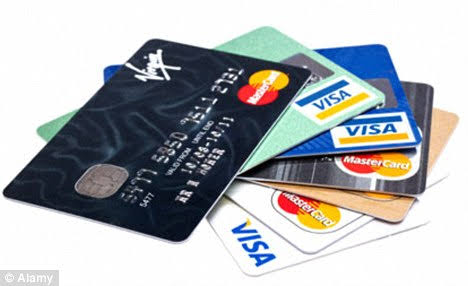
\includegraphics[scale=0.3,angle=360]{img1.jpg}
\caption{Credit Cards}
\end{center}
\end{figure}









\begin{itemize}
\item Type of electronic payment system that involves the use of a plastic card with a magnetic stripe that retains information of the cardholder’s credit account made with a bank.
\item  Printed bank card number with the ISO 7812 numbering standard. 
\item Universal size: 85.60 mm * 53.98 mm.

\end{itemize}
\end{frame}


%%%%%%%%%%%%%%%%%%%%%%%%%%%%%%%%%%%%%%%%%%%%%%%%%%%%%%%
\begin{frame}
\frametitle{Working of CREDIT Cards :} 
\begin{figure}[h]
\begin{center}
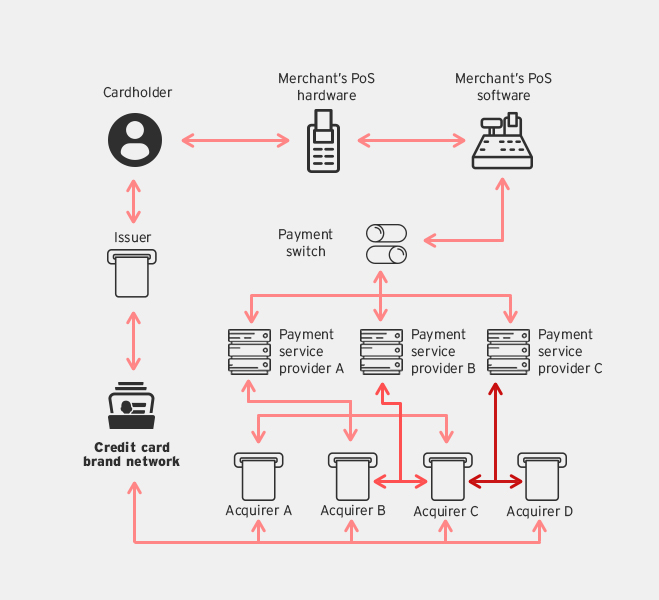
\includegraphics[scale=0.18,angle=360]{img2.jpg}
\caption{Credit-card payment system }
\end{center}
\end{figure}

\begin{itemize}
\item Consumer
\item Merchant
\item Issuer
\item Acquirer
\item Card brand
\item Payment Service Provider


\end{itemize}
\end{frame}
%%%%%%%%%%%%%%%%%%%%%%%%%%%%%%%%%%%%%%%%%%%%%%%%%%%%%%%
\begin{frame}
\frametitle{EMV}
\begin{figure}[h]
\begin{center}
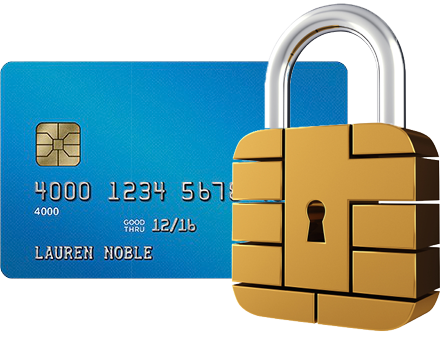
\includegraphics[scale=0.2,angle=360]{img3.png}
\caption{Europay Master Card and Visa}
\end{center}
\end{figure}
\begin{itemize}
\item EMV cards are smart cards that store customers data on integrated circuits in addition to magnetic stripes .
\item Chip and Pin Aunthentication method.
\item It can be read by radio-frequency identification (RFID) technology. 


\end{itemize}
\end{frame}
%%%%%%%%%%%%%%%%%%%%%%%%%%%%%%%%%%%%%%%%%%%%%






\begin{frame}
\frametitle{Advantages}
\begin{itemize}
\item The introduction of dynamic data is what makes EMV cards so effective.
\item Reset mechanism through card interface functions.
\item It supports various verification methods such as online pin, offline pin , digital signiture.
\item Extremely difficult to duplicate the data which are stored in chip. 
\item Silver lining technology to reduce the pos frauds.
\end{itemize}
\end{frame}
%%%%%%%%%%%%%%%%%%%%%%%%%%%




\begin{frame}
\frametitle{NFC Payment System}
\begin{figure}[h]
\begin{center}
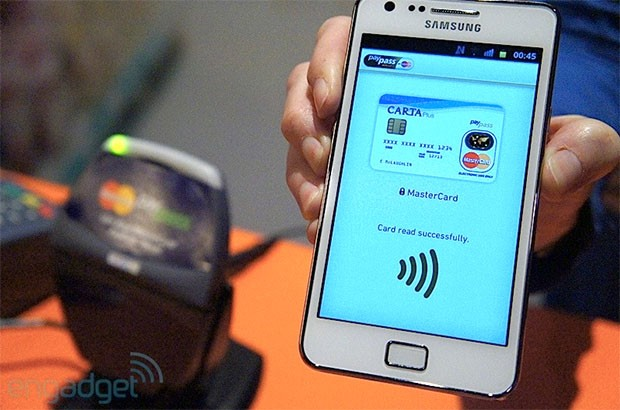
\includegraphics[scale=0.2,angle=360]{nfc1.jpg}
\caption{Near Field Communication}
\end{center}
\end{figure}







\begin{itemize}
\item NFC is the technology that enables contactless payments.
\item NFC is a set of communication protocols that enable two electronic devices, smartphone and payment terminal to establish communication by bringing them within 4 cm (1.6 in) of each other.
\item NFC offers a low-speed connection set up used for social networking, for sharing contacts, photos, videos or files.
\end{itemize}
\end{frame}
%%%%% FIGURE CODE
\begin{frame}
\frametitle{FEATURES}
\begin{itemize}
\item Support devices with single or multiple NFC adapters.
\item Support communication with active (readers, phones) and passive (smart cards, tags) devices.
\item Allow NFC handover to Bluetooth or WiFi.
\item Allow card emulation with secure element or host card emulation.
\end{itemize}
\end{frame}


%%%%%%%%%%%%%%%%%%%%%%%%%%%%%%%%%%%%%%%%%%%%

\begin{frame}
\frametitle{APPLE-PAY}

\begin{figure}[h]
\begin{center}
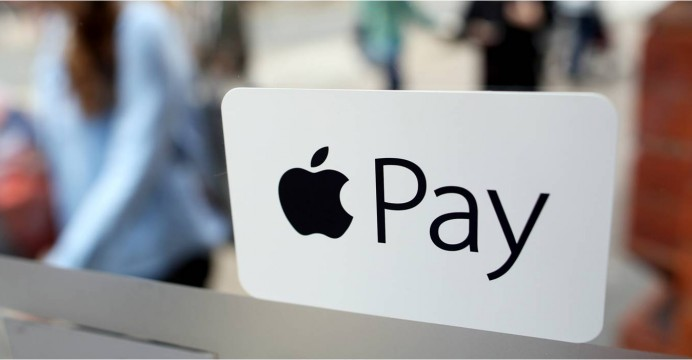
\includegraphics[scale=0.2,angle=360]{apple1.jpg}
\caption{Apple-Pay}
\end{center}
\end{figure}
\begin{itemize}
\item Apple Pay is a mobile payment and digital wallet service by Apple Inc. 
\item Supported Device:
           \begin{itemize}
	       \item iPhone 6, 6 Plus, iPhone 6S, 6S Plus, iPhone 7, 7 Plus, iPhone SE, and later.. 
           \item iPad Air 2, iPad Pro and iPad Mini 3 and later..
           \item  Apple Watch-compatible devices.
           \item macbooks with mac'OS Sierra.
           \end{itemize}
\end{itemize}       



\end{frame}


%%%%%%%%%%%%%%%%%%%%%%%%%%%%%%%%%%%%%%%%%%%%
\begin{frame}
\frametitle{Apple-Pay Working} 
\begin{figure}[h]
\begin{center}
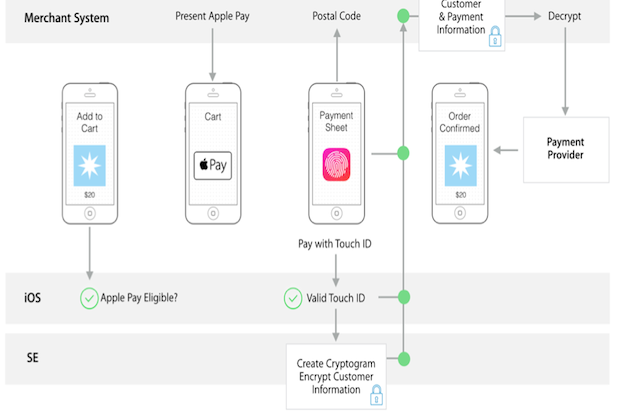
\includegraphics[scale=0.4,angle=360]{apple2.png}
\caption{Apple-Pay Working}
\end{center}
\end{figure}

\end{frame}
%%%%%%%%%%%%%%%%%%%%%%%%%%%%%%%%%%%%%%%%%%%%%%%%
\begin{frame}
\frametitle{Ways to use Apple-Pay }
\begin{itemize}
\item  Set up Apple Pay on iPhone.
\item  Set up Apple Pay on Apple Watch.
\item  Using Apple Pay.
\item  Update and remove.
\item  Is it safe?

\end{itemize}

\end{frame}

%%%%%%%%%%%%%%%%%%%%%%%%%%%%%%%%%%%%%%%%%%







\begin{frame}
\frametitle{E-VALLET}
\begin{figure}[h]
\begin{center}
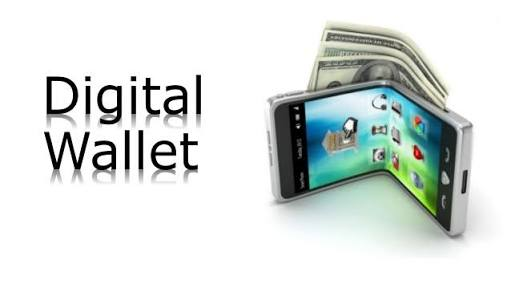
\includegraphics[scale=0.2,angle=360]{vallet1.jpg}
\end{center}
\end{figure}






\begin{itemize}
\item A digital wallet refers to an electronic device that allows an individual to make electronic transactions.
\item A digital wallet has both a software and information component.
\item The software provides security and encryption for the personal information and for the actual transaction.
\item The information component consists of your shipping address, billing address, payment methods, and other credintial information.

\end{itemize}
\end{frame}
%%%%%%%%%%%%%%%%%%%%%%%%%%%%%%%%%%%%%%%%%%KISS
\begin{frame}
\frametitle{Statistics and Prediction}

\begin{figure}[h]
\begin{center}
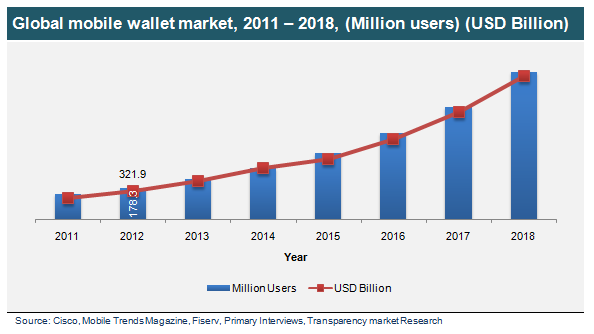
\includegraphics[scale=0.3,angle=360]{vallet4.png}
\end{center}
\end{figure}

\begin{figure}[h]
\begin{center}
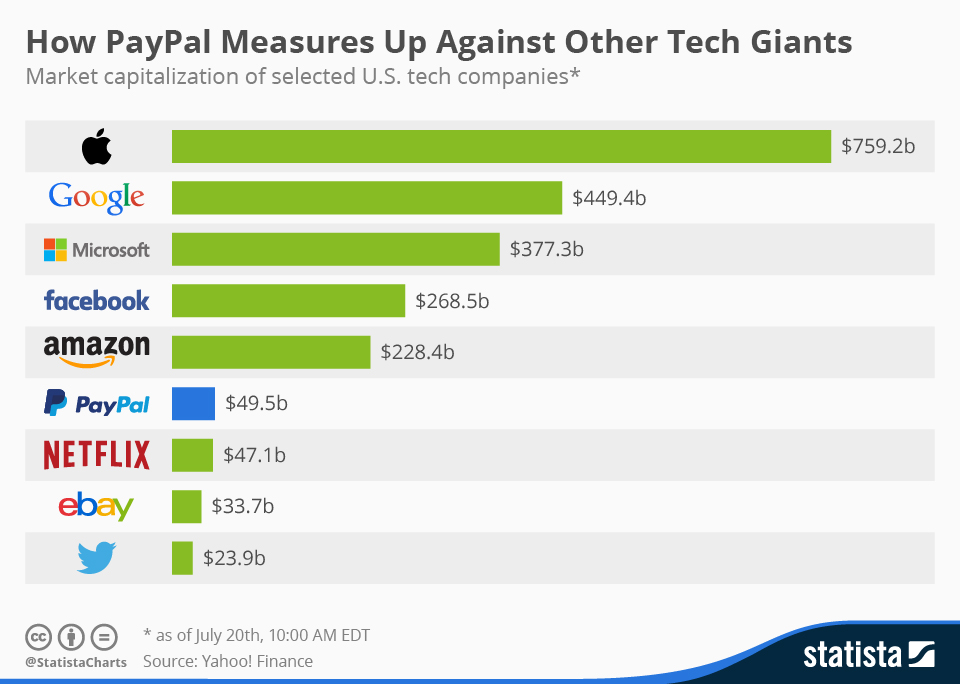
\includegraphics[scale=0.2,angle=360]{vallet6.jpg}
\end{center}
\end{figure}



\end{frame}
%%%%%%%%%%%%%%%%%%%%%%%%%%%%%%%%%%%%%%%%%%%%

%%%%%%%%%%%%%%%%%%%%%%%%%%%%%%%%%%%%%%%%%%%%%
%%%%%%%%%%%%%%%%%%%%%%%
\begin{frame}
\frametitle{Conclusion}
\begin{itemize}

\item The unique combination of a NFC based mobile wallet and card provides flexibility, convenience and financial control to consumers, in addition to encouraging the use of the latest technology.
\item Consumer education remains an area of acute interest for banks to implement use of Eco friendly financial services.
\item Adopting Mobile based, Card base solution will reduce the physical printing money, which will have greater impact on economy growth.
\item Green IT banking based practices in banking are critical to the future development of the nation and national progress.




\end{itemize}
\end{frame}
%%%%%%%%%%%%%%%%%%%%%%% NEED CHANGE

%%%%%%%%%%%%%%%%%%%%%%%%%%%%%%%%%%%%5
\begin{frame}
\frametitle{Refrences}
\begin{enumerate}
\item  K.V. Kuganathan, Gihan N. Wikramanayake ,``Next Generation Smart Transaction Touch Points'',IEEE 2014.\\
\item  Oludele Ogundele, Pavol Zavarsky, Ron Ruhl,``The Implementation of a full EMV Smartcard for a Point-of-Sale Transaction", IEEE 2012.\\
\item Luca Mainetti, Luigi Patrono, Roberto Vergallo,``IDA-Pay: an innovative micro-payment system based on NFC technology for Android mobile devices",IEEE 2012.\\ 
\item Sana Nseir , Nael Hirzallah, Musbah Aqel,``A Secure Mobile Payment System using QR Code",IEEE 2013. \\
\item Mia Olsen, Jonas Hedman and Ravi Vatrapu,``E-wallet Properties",IEEE 2011.\\

\end{enumerate}

\end{frame}




\begin{frame}
\frametitle{Any Questions}

\begin{figure}[h]
         \begin{center}

\includegraphics[scale=0.4,angle=360]{questions.jpg}
\end{center}
\end{figure}
\end{frame}

%%%%%%%%%%%%%%%%%%%%%%%%%%%%%%%

\begin{frame}
\begin{figure}[h]
         \begin{center}

\includegraphics[scale=0.2,angle=360]{thanks.jpg}
\end{center}
\end{figure}

\end{frame}




%%%%%%%
%%%%%%%%%%%%%%%%%
%%%%%%%%%%%%%%%%%%%%%%%%%%%%%%%%%
%\begin{frame}
%\frametitle{References}
%\setbeamertemplate{bibliography item}{\insertbiblabel}
%\renewcommand{\refname}{}
%\bibliography{ref}


% K.V. Kuganathan, Gihan N. Wikramanayake, National Development Bank PLC·University of Colombo School of Computing,SriLanka,``Next Generation Smart Transaction Touch Points",ICT 2014.


%\end{frame}
%%%%%%%%%%%%
%%%%%%%%%%%%%%%
%%%%%%%%%%%%%%%%%%%%%
\end{document}
